%%%%%%%%%%%%%%%%%%%%%%%%%%%%%%%%%%%%%%%%%
% Thin Sectioned Essay
% LaTeX Template
% Version 1.0 (3/8/13)
%
% This template has been downloaded from:
% http://www.LaTeXTemplates.com
%
% Original Author:
% Nicolas Diaz (nsdiaz@uc.cl) with extensive modifications by:
% Vel (vel@latextemplates.com)
%
% License:
% CC BY-NC-SA 3.0 (http://creativecommons.org/licenses/by-nc-sa/3.0/)
%
%%%%%%%%%%%%%%%%%%%%%%%%%%%%%%%%%%%%%%%%%

%----------------------------------------------------------------------------------------
%	PACKAGES AND OTHER DOCUMENT CONFIGURATIONS
%----------------------------------------------------------------------------------------

\documentclass[a4paper, 11pt]{article} % Font size (can be 10pt, 11pt or 12pt) and paper size (remove a4paper for US letter paper)

\usepackage[protrusion=true,expansion=true]{microtype} % Better typography
\usepackage{graphicx} % Required for including pictures
\usepackage{wrapfig} % Allows in-line images

\usepackage{mathpazo} % Use the Palatino font
\usepackage[T1]{fontenc} % Required for accented characters
\linespread{1.05} % Change line spacing here, Palatino benefits from a slight increase by default

\makeatletter
\renewcommand\@biblabel[1]{\textbf{#1.}} % Change the square brackets for each bibliography item from '[1]' to '1.'
\renewcommand{\@listI}{\itemsep=0pt} % Reduce the space between items in the itemize and enumerate environments and the bibliography

\renewcommand{\maketitle}{ % Customize the title - do not edit title and author name here, see the TITLE block below
\begin{flushright} % Right align
{\LARGE\@title} % Increase the font size of the title

\vspace{50pt} % Some vertical space between the title and author name

{\large\@author} % Author name
\\\@date % Date

\vspace{40pt} % Some vertical space between the author block and abstract
\end{flushright}
}

%----------------------------------------------------------------------------------------
%	TITLE
%----------------------------------------------------------------------------------------

\title{\textbf{Research Internship 1st Report}\\ % Title
Reinforcement Learning Overview \\and Tactile Reward Setting} % Subtitle

\author{\textsc{Tianming Qiu} % Author
\\{\textit{Institute for Cognitive Systems}}} % Institution

\date{\today} % Date

%----------------------------------------------------------------------------------------

\begin{document}


\maketitle % Print the title section


\section{Reinforcement Learning Overview} 
Some basic knowledges from Sutton's \textit{Reinforcement learning: An introduction}\cite {sutton1998reinforcement} and UCL course on RL from David Silver. 

\subsection{Markov Decision Process}
A Markov decision process is a discrete-time state transition system. It can be described formally with 5 components as a 5-tuple $(\mathcal{S,A,P}, r,\gamma)$. $\mathcal{S}$: States

\textbf{$\mathcal{A}$: Action}\quad 
A small finite set includes 'drive east','drive west', 'drive north' as well as 'drive south'.

\textbf{$\mathcal{S}$: Transition probability}\quad 
The transition probabilities describe the dynamics of the world. They play the role of the next-state function in a problem-solving search, except that every state is thought to be a possible consequence of taking an action in a state. So, we specify, for each state $s_{t}$ and action $a_{t}$, the probability that the next state will be $s_{t+1}$. 
Now we just model the transition probability as the simplest one: All of them equal to one. That means if and only if Epuck takes a specific action (e.g. turn right) at the current action, it will transit into a definitely deterministic state.

\textbf{$r$: Reward}\quad  In this model we will assign a reward '+10' at the destination state and '0' at the other states. 
Also at the 'blind alley' it will get a very poor reward such as '-100'.

\textbf{$\gamma$}  \quad It is a discout factor here we select as 0.9.
\subsection{Model based dynamic programming}
\begin{enumerate}
\item Value iteration
\item Policy iteration
\end{enumerate}
\subsection{Model free Reinforcement learning: MC and TD}
\subsection{Q learning and Sarsa}
\subsubsection{Q}
\begin{center}\textbf{Q-learning: An off-policy TD control algorithm}

\fbox{\parbox{\textwidth}{Initialize $Q(s,a)$, $\forall s \in \mathcal{S}$, $\forall a \in \mathcal{A}$, arbitrarily, and $Q($terminal-state,$\cdot)=0$

Repeat (for each episode):

\quad\quad Initialize $S$

\quad\quad Repeat (for each step of episode):

\quad\quad \quad\quad Choose $A$ from $S$ using policy derived from $Q$ (e.g., $\epsilon$-greedy)

\quad\quad \quad\quad Take action $A$, observe $R$, $S'$

\quad\quad \quad\quad $Q(S_t,A_t)\leftarrow Q(S_t,A_t)+ \alpha [ R_{t+1} + \gamma \max \limits_{a}Q(S_{t+1},a)-Q(S_t,A_t)]$

\quad\quad \quad\quad $S\leftarrow S'$

\quad\quad Until $S$ is terminal
}}

\end{center}
\subsection{DQN}
%------------------------------------------------

\section*{Section Name}

Cras gravida, est vel interdum euismod, tortor mi lobortis mi, quis adipiscing elit lacus ut orci. Phasellus nec fringilla nisi, ut vestibulum neque. Aenean non risus eu nunc accumsan condimentum at sed ipsum.
%\begin{wrapfigure}{l}{0.4\textwidth} % Inline image example
%\begin{center}
%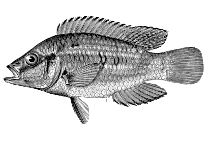
\includegraphics[width=0.38\textwidth]{fish.png}
%\end{center}
%\caption{Fish}
%\end{wrapfigure}
Aliquam fringilla non diam sed varius. Suspendisse tellus felis, hendrerit non bibendum ut, adipiscing vitae diam. Lorem ipsum dolor sit amet, consectetur adipiscing elit. Nulla lobortis purus eget nisl scelerisque, commodo rhoncus lacus porta. Vestibulum vitae turpis tincidunt, varius dolor in, dictum lectus. Aenean ac ornare augue, ac facilisis purus. Sed leo lorem, molestie sit amet fermentum id, suscipit ut sem. Vestibulum orci arcu, vehicula sed tortor id, ornare dapibus lorem. Praesent aliquet iaculis lacus nec fermentum. Morbi eleifend blandit dolor, pharetra hendrerit neque ornare vel. Nulla ornare, nisl eget imperdiet ornare, libero enim interdum mi, ut lobortis quam velit bibendum nibh.

Morbi tempor congue porta. Proin semper, leo vitae faucibus dictum, metus mauris lacinia lorem, ac congue leo felis eu turpis. Sed nec nunc pellentesque, gravida eros at, porttitor ipsum. Praesent consequat urna a lacus lobortis ultrices eget ac metus. In tempus hendrerit rhoncus. Mauris dignissim turpis id sollicitudin lacinia. Praesent libero tellus, fringilla nec ullamcorper at, ultrices id nulla. Phasellus placerat a tellus a malesuada.

%------------------------------------------------

\section*{Conclusion}

Fusce in nibh augue. Cum sociis natoque penatibus et magnis dis parturient montes, nascetur ridiculus mus. In dictum accumsan sapien, ut hendrerit nisi. Phasellus ut nulla mauris. Phasellus sagittis nec odio sed posuere. Vestibulum porttitor dolor quis suscipit bibendum. Mauris risus lectus, cursus vitae hendrerit posuere, congue ac est. Suspendisse commodo eu eros non cursus. Mauris ultrices venenatis dolor, sed aliquet odio tempor pellentesque. Duis ultricies, mauris id lobortis vulputate, tellus turpis eleifend elit, in gravida leo tortor ultricies est. Maecenas vitae ipsum at dui sodales condimentum a quis dui. Nam mi sapien, lobortis ac blandit eget, dignissim quis nunc.

\begin{enumerate}
\item First numbered list item
\item Second numbered list item
\end{enumerate}

Donec luctus tincidunt mauris, non ultrices ligula aliquam id. Sed varius, magna a faucibus congue, arcu tellus pellentesque nisl, vel laoreet magna eros et magna. Vivamus lobortis elit eu dignissim ultrices. Fusce erat nulla, ornare at dolor quis, rhoncus venenatis velit. Donec sed elit mi. Sed semper tellus a convallis viverra. Maecenas mi lorem, placerat sit amet sem quis, adipiscing tincidunt turpis. Cras a urna et tellus dictum eleifend. Fusce dignissim lectus risus, in bibendum tortor lacinia interdum.

%----------------------------------------------------------------------------------------
%	BIBLIOGRAPHY
%----------------------------------------------------------------------------------------

\bibliographystyle{unsrt}

\bibliography{sample}

%----------------------------------------------------------------------------------------

\end{document}